\subsection{Packet Loss and Delays}

When the arrival rate of packets at a router exceeds the output link capacity, the packets wait in a buffer queue for transmission.
A packet is dropped (lost) if there is no available buffer space in the queue when it arrives.
A lost packet may be retransmitted by the previous node, the end system source or not at all.
Nodal delay \( d_{\text{nodal}} \) is the delay of packets at a node in a network.

\begin{equation*}
  d_{\text{nodal}} = d_{\text{proc}} + d_{\text{queue}} + d_{\text{trans}} + d_{\text{prop}}
\end{equation*}

\begin{itemize}
  \item Nodal processing delay (\( d_{\text{proc}} \))
  \begin{itemize}
    \item Time spent checking bit errors and determining output link
    \item Typically less than a millisecond
  \end{itemize}
  \item Queueing delay (\( d_{\text{queue}} \))
  \begin{itemize}
    \item Time spent waiting at output link for transmission
    \item Dependent upon congestion level at link/router
  \end{itemize}
  \item Transmission delay (\( d_{\text{trans}} \))
  \begin{itemize}
    \item Time spent placing packet onto output link
    \item For a packet of length \(L\)~\si{\bit} and link of bandwidth \(R\)~\si{\bit\per\second}, \( d_{\text{trans}} = \frac{L}{R} \)~\si{\second}
  \end{itemize}
  \item Propagation delay (\( d_{\text{prop}} \))
  \begin{itemize}
    \item Time spent travelling through output link to next node
    \item For a link of length \(d\)~\si{\metre} and a propagation speed through the link medium of \(s\)~\si{\metre\per\second}, \( d_{\text{prop}} = \frac{d}{s} \)~\si{\second}
  \end{itemize}
\end{itemize}

Throughput is the rate at which bits are transferred between sender and receiver.
Throughput can be measured as instantaneous throughput at a specific point in time or average throughput over a longer period of time.
The average end-to-end throughput is determined by the link with the lowest capacity.
A link on an end-to-end path that constrains the throughput is known as a `bottleneck link'.

\subsection{Protocols}

Network protocols define a set of guidelines that allow network devices to communicate effectively.
A protocol defines the sequence of messages that should be exchanged and the format of the data in the messages.
Protocols are implemented by a pair of software modules in the sending and receiving systems.

A transport protocol transmits a message from a sender to a receiver.
A process that wishes to send a message passes it to the transport protocol module.
The software divides the message into packets, which are then transmitted using the network protocol.
Inverse operations are performed by the receiver to reconstruct the message.

\begin{figure}[htp]
  \centering
  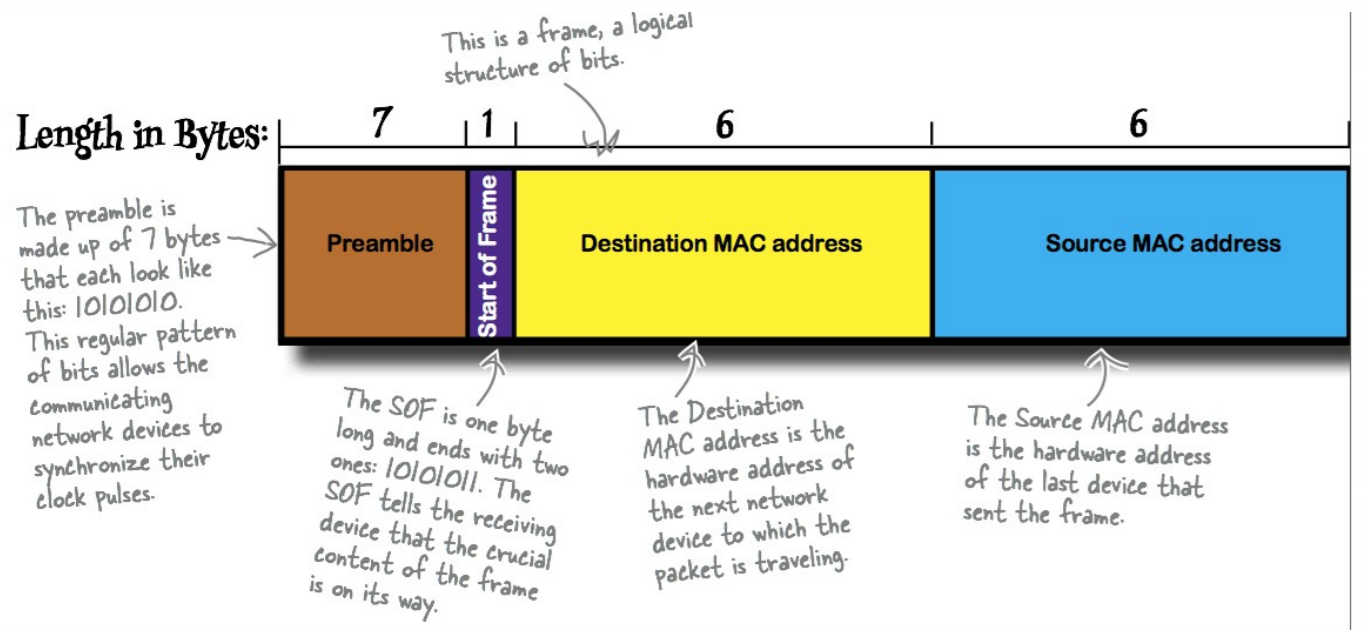
\includegraphics[width=15cm]{unit-16/figures/frame-part-1.png}
  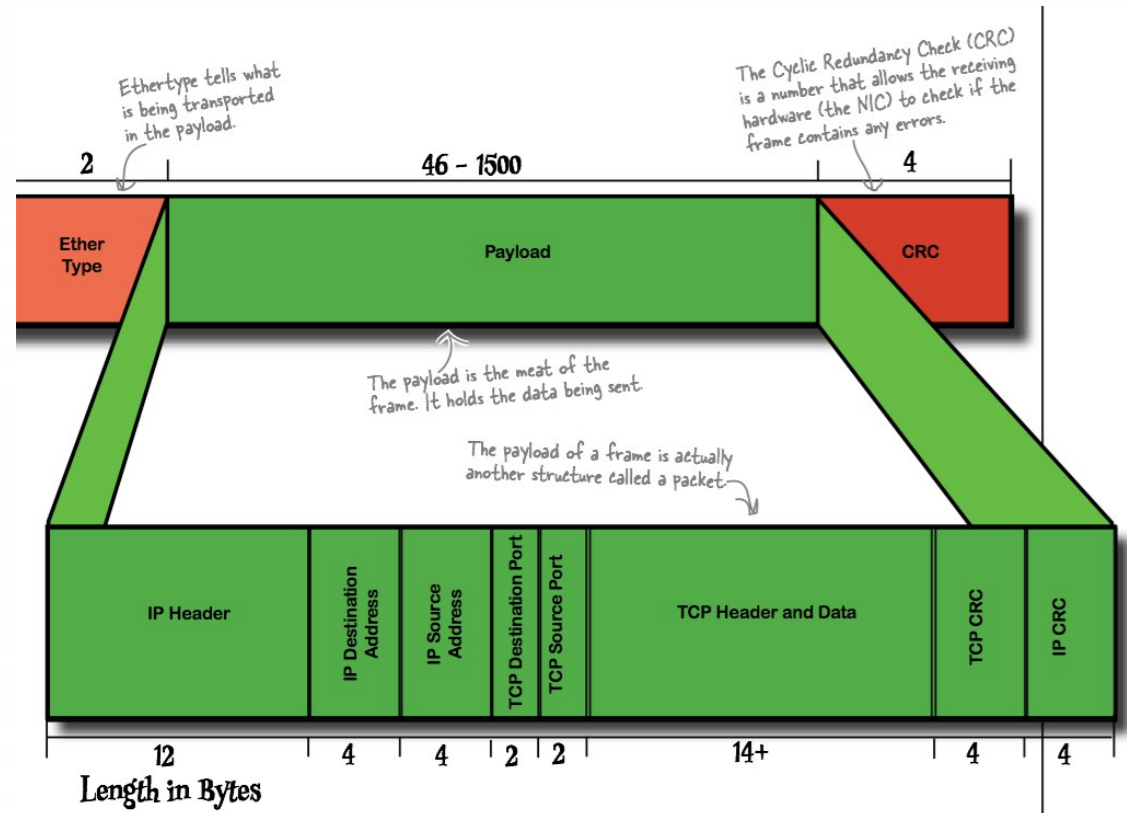
\includegraphics[width=15cm]{unit-16/figures/frame-part-2.png}
  \caption*{The structure of a packet frame.}
\end{figure}

\subsection{Protocol Layers and Encapsulation}

Network software is arranged in a hierarchy of layers, in which each layer presents an interface to the layer above.
Each layer accepts an item of data in a specified format from the layer above.
It applies a transformation to the data in order to encapsulate it.
The data is passed to the layer below.
Layers communicate with those directly above and below through procedure calls.
Every computer in a network must have these layers.

A complete set of protocol layers is known as a `protocol suite' or `protocol stack'.
Each layer adds a header to the data before it is sent.

\subsection{Open Systems Interconnection (OSI) Model}

The Open Systems Interconnection (OSI) model is a conceptual protocol stack model.
Its layers from highest to lowest are
\begin{itemize}
  \item application,
  \item presentation,
  \item session,
  \item transport,
  \item network,
  \item (data) link, and
  \item physical.
\end{itemize}

Data are passed down through the layers in the source end system and across the network via physical connections.
Switches and routers use the data link and network layers to route the data through the network.
When the data arrive at the end system, they are passed up through the layers and are reconstructed.

\begin{table}[htp]
  \centering
  \caption*{The layers of the OSI model.}
  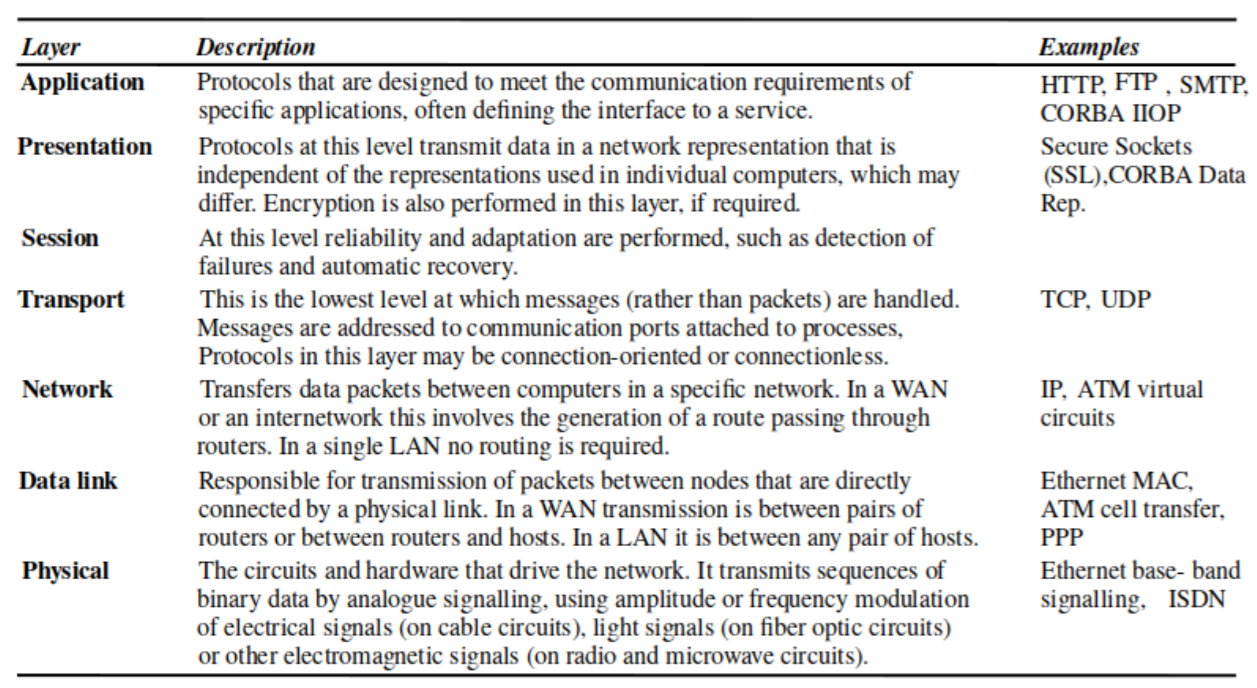
\includegraphics[width=15cm]{unit-16/figures/layer-summary.png}
\end{table}

Protocol layering simplifies and generalises the software interfaces that access communication services.
However, they reduce the performance of the network.
A total of \(N\) protocol layers results in \(N\) control transfers for each message at an end system, and \(N\) copies of the data due to encapsulation.
Thus, the data transfer rate may be much slower than the available network bandwidth.

The five-layer protocol stack used by the Internet differs from the seven-layer OSI model.
Its layers from highest to lowest are
\begin{itemize}
  \item application,
  \item transport,
  \item network,
  \item link, and
  \item physical.
\end{itemize}
The application, presentation and session layers of the OSI model are not clearly distinguished in the Internet protocol stack, and are instead all part of a single application layer.
Applications are responsible for deciding how to handle these protocols.
The session layer is integrated with the transport layer.

\subsection{Large Messages and Message Consistency}

An Ethernet frame can only hold \SI{1500}{\byte} of data.
Messages larger than this limit must be broken into packets.
Message consistency and reliable data transfer are achieved by communicating via the Transmission Control Protocol (TCP).
If there are errors in the packets, the receiver notifies the sender, and those packets are sent again.
If the message is a single long packet, there may be issues due to poor connection.

Packets may not be received in the same order that they are sent.
Each packet contains a sequence number so that they can be reordered correctly.

\subsection{Ports and Addressing}

The responsibility of the transport layer is to provide a network-independent message transfer service between pairs of network ports.
The destination ports at a host computer are defined by software and are attached to processes.
Port~\num{25} is used for email.

The transport layer delivers messages to destination specified by transport addresses.
A transport address comprises a network address and a port number.
In the Internet, every host system is assigned an Internet Protocol (IP) address that identifies it and the subnet to which it is connected.

\subsection{Datagram Packet Delivery}

In datagram packet delivery, it is the responsibility of the receiver to indicate if there is a problem with transmission.
The network retains no information after it has been delivered.
The sequence of packets may take different routes from hose to destination, so they may arrive out of sequence.
Datagrams contain the full network addresses of the source and destination.
The network layer of the Internet uses datagram delivery.

A link-layer switch accesses the data link layer of a packet to determine the next link to which the packet must be sent.
A router is a three-layer switch.
It accesses the network layer of the packet in order to route the packet to the destination host.
